% Created by tikzDevice version 0.12 on 2019-02-08 13:14:33
% !TEX encoding = UTF-8 Unicode
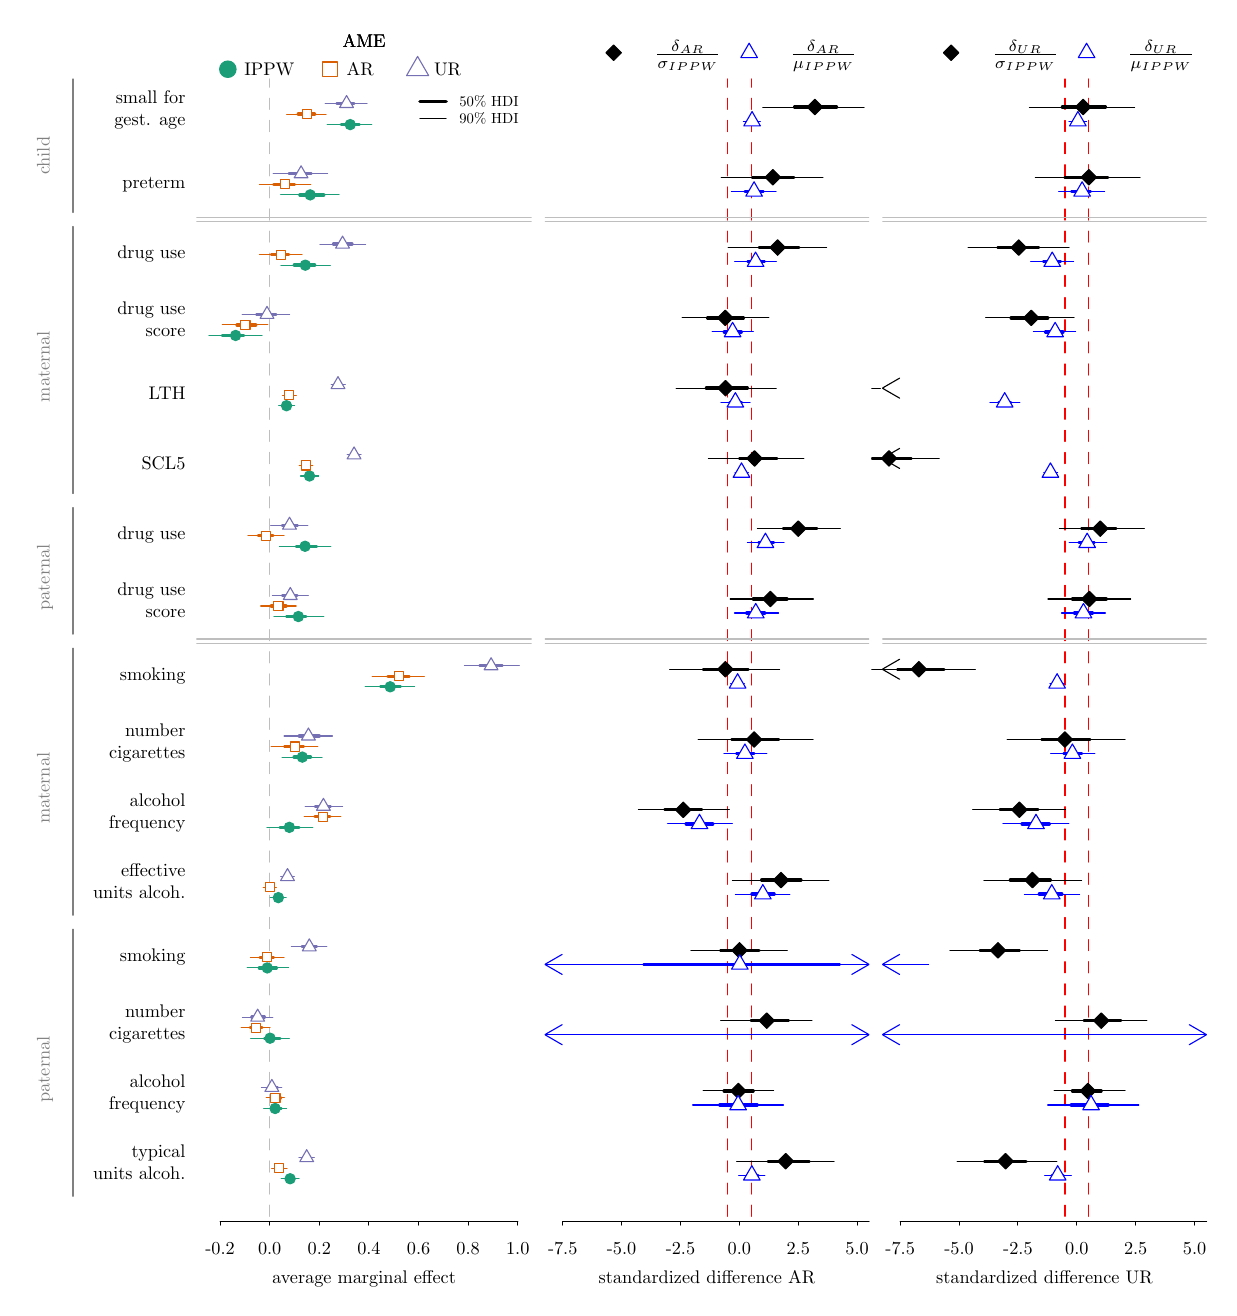
\begin{tikzpicture}[x=1pt,y=1pt]
\definecolor{fillColor}{RGB}{255,255,255}
\path[use as bounding box,fill=fillColor,fill opacity=0.00] (0,0) rectangle (426.79,455.24);
\begin{scope}
\path[clip] (  0.00, 23.76) rectangle ( 60.97,443.36);
\definecolor{drawColor}{RGB}{0,0,0}

\node[text=drawColor,anchor=base east,inner sep=0pt, outer sep=0pt, scale=  0.66] at ( 57.01,427.78) {small for};

\node[text=drawColor,anchor=base east,inner sep=0pt, outer sep=0pt, scale=  0.66] at ( 57.01,419.86) {gest. age};

\node[text=drawColor,anchor=base east,inner sep=0pt, outer sep=0pt, scale=  0.66] at ( 57.01,397.11) {preterm};

\node[text=drawColor,anchor=base east,inner sep=0pt, outer sep=0pt, scale=  0.66] at ( 57.01,371.71) {drug use};

\node[text=drawColor,anchor=base east,inner sep=0pt, outer sep=0pt, scale=  0.66] at ( 57.01,351.60) {drug use};

\node[text=drawColor,anchor=base east,inner sep=0pt, outer sep=0pt, scale=  0.66] at ( 57.01,343.68) {score};

\node[text=drawColor,anchor=base east,inner sep=0pt, outer sep=0pt, scale=  0.66] at ( 57.01,320.92) {LTH};

\node[text=drawColor,anchor=base east,inner sep=0pt, outer sep=0pt, scale=  0.66] at ( 57.01,295.53) {SCL5};

\node[text=drawColor,anchor=base east,inner sep=0pt, outer sep=0pt, scale=  0.66] at ( 57.01,270.14) {drug use};

\node[text=drawColor,anchor=base east,inner sep=0pt, outer sep=0pt, scale=  0.66] at ( 57.01,250.02) {drug use};

\node[text=drawColor,anchor=base east,inner sep=0pt, outer sep=0pt, scale=  0.66] at ( 57.01,242.10) {score};

\node[text=drawColor,anchor=base east,inner sep=0pt, outer sep=0pt, scale=  0.66] at ( 57.01,219.35) {smoking};

\node[text=drawColor,anchor=base east,inner sep=0pt, outer sep=0pt, scale=  0.66] at ( 57.01,199.24) {number};

\node[text=drawColor,anchor=base east,inner sep=0pt, outer sep=0pt, scale=  0.66] at ( 57.01,191.32) {cigarettes};

\node[text=drawColor,anchor=base east,inner sep=0pt, outer sep=0pt, scale=  0.66] at ( 57.01,173.84) {alcohol };

\node[text=drawColor,anchor=base east,inner sep=0pt, outer sep=0pt, scale=  0.66] at ( 57.01,165.92) {frequency};

\node[text=drawColor,anchor=base east,inner sep=0pt, outer sep=0pt, scale=  0.66] at ( 57.01,148.45) {effective};

\node[text=drawColor,anchor=base east,inner sep=0pt, outer sep=0pt, scale=  0.66] at ( 57.01,140.53) {units alcoh.};

\node[text=drawColor,anchor=base east,inner sep=0pt, outer sep=0pt, scale=  0.66] at ( 57.01,117.78) {smoking};

\node[text=drawColor,anchor=base east,inner sep=0pt, outer sep=0pt, scale=  0.66] at ( 57.01, 97.66) {number};

\node[text=drawColor,anchor=base east,inner sep=0pt, outer sep=0pt, scale=  0.66] at ( 57.01, 89.74) {cigarettes};

\node[text=drawColor,anchor=base east,inner sep=0pt, outer sep=0pt, scale=  0.66] at ( 57.01, 72.27) {alcohol };

\node[text=drawColor,anchor=base east,inner sep=0pt, outer sep=0pt, scale=  0.66] at ( 57.01, 64.35) {frequency};

\node[text=drawColor,anchor=base east,inner sep=0pt, outer sep=0pt, scale=  0.66] at ( 57.01, 46.88) {typical};

\node[text=drawColor,anchor=base east,inner sep=0pt, outer sep=0pt, scale=  0.66] at ( 57.01, 38.96) {units alcoh.};
\definecolor{drawColor}{gray}{0.50}

\path[draw=drawColor,line width= 0.4pt,line join=round,line cap=round] ( 16.37,436.71) -- ( 16.37,388.46);

\path[draw=drawColor,line width= 0.4pt,line join=round,line cap=round] ( 16.37,383.38) -- ( 16.37,286.89);

\path[draw=drawColor,line width= 0.4pt,line join=round,line cap=round] ( 16.37,281.81) -- ( 16.37,236.10);

\path[draw=drawColor,line width= 0.4pt,line join=round,line cap=round] ( 16.37,231.02) -- ( 16.37,134.53);

\path[draw=drawColor,line width= 0.4pt,line join=round,line cap=round] ( 16.37,129.45) -- ( 16.37, 32.95);

\node[text=drawColor,rotate= 90.00,anchor=base,inner sep=0pt, outer sep=0pt, scale=  0.66] at (  7.90,408.93) {child};

\node[text=drawColor,rotate= 90.00,anchor=base,inner sep=0pt, outer sep=0pt, scale=  0.66] at (  7.90,332.75) {maternal};

\node[text=drawColor,rotate= 90.00,anchor=base,inner sep=0pt, outer sep=0pt, scale=  0.66] at (  7.90,256.57) {paternal};

\node[text=drawColor,rotate= 90.00,anchor=base,inner sep=0pt, outer sep=0pt, scale=  0.66] at (  7.90,180.39) {maternal};

\node[text=drawColor,rotate= 90.00,anchor=base,inner sep=0pt, outer sep=0pt, scale=  0.66] at (  7.90, 78.81) {paternal};
\end{scope}
\begin{scope}
\path[clip] (  0.00,  0.00) rectangle (426.79,455.24);
\definecolor{drawColor}{RGB}{0,0,0}

\path[draw=drawColor,line width= 0.4pt,line join=round,line cap=round] ( 69.54, 23.76) -- (177.09, 23.76);

\path[draw=drawColor,line width= 0.4pt,line join=round,line cap=round] ( 69.54, 23.76) -- ( 69.54, 22.55);

\path[draw=drawColor,line width= 0.4pt,line join=round,line cap=round] ( 87.46, 23.76) -- ( 87.46, 22.55);

\path[draw=drawColor,line width= 0.4pt,line join=round,line cap=round] (105.39, 23.76) -- (105.39, 22.55);

\path[draw=drawColor,line width= 0.4pt,line join=round,line cap=round] (123.31, 23.76) -- (123.31, 22.55);

\path[draw=drawColor,line width= 0.4pt,line join=round,line cap=round] (141.24, 23.76) -- (141.24, 22.55);

\path[draw=drawColor,line width= 0.4pt,line join=round,line cap=round] (159.16, 23.76) -- (159.16, 22.55);

\path[draw=drawColor,line width= 0.4pt,line join=round,line cap=round] (177.09, 23.76) -- (177.09, 22.55);

\node[text=drawColor,anchor=base,inner sep=0pt, outer sep=0pt, scale=  0.66] at ( 69.54, 11.88) {-0.2};

\node[text=drawColor,anchor=base,inner sep=0pt, outer sep=0pt, scale=  0.66] at ( 87.46, 11.88) {0.0};

\node[text=drawColor,anchor=base,inner sep=0pt, outer sep=0pt, scale=  0.66] at (105.39, 11.88) {0.2};

\node[text=drawColor,anchor=base,inner sep=0pt, outer sep=0pt, scale=  0.66] at (123.31, 11.88) {0.4};

\node[text=drawColor,anchor=base,inner sep=0pt, outer sep=0pt, scale=  0.66] at (141.24, 11.88) {0.6};

\node[text=drawColor,anchor=base,inner sep=0pt, outer sep=0pt, scale=  0.66] at (159.16, 11.88) {0.8};

\node[text=drawColor,anchor=base,inner sep=0pt, outer sep=0pt, scale=  0.66] at (177.09, 11.88) {1.0};
\end{scope}
\begin{scope}
\path[clip] ( 60.97,  0.00) rectangle (182.91,455.24);
\definecolor{drawColor}{RGB}{0,0,0}

\node[text=drawColor,anchor=base,inner sep=0pt, outer sep=0pt, scale=  0.66] at (121.54,  1.58) {average marginal effect};
\end{scope}
\begin{scope}
\path[clip] ( 60.97, 23.76) rectangle (182.12,443.36);
\definecolor{drawColor}{RGB}{190,190,190}

\path[draw=drawColor,line width= 0.4pt,dash pattern=on 4pt off 4pt ,line join=round,line cap=round] ( 87.46, 17.72) --
	( 87.46,436.71);
\definecolor{drawColor}{RGB}{27,158,119}

\path[draw=drawColor,line width= 1.2pt,line join=round,line cap=round] (113.25,420.21) -- (119.87,420.21);

\path[draw=drawColor,line width= 1.2pt,line join=round,line cap=round] ( 98.36,394.81) -- (106.99,394.81);

\path[draw=drawColor,line width= 1.2pt,line join=round,line cap=round] ( 96.34,369.42) -- (103.69,369.42);

\path[draw=drawColor,line width= 1.2pt,line join=round,line cap=round] ( 70.30,344.02) -- ( 78.08,344.02);

\path[draw=drawColor,line width= 1.2pt,line join=round,line cap=round] ( 92.31,318.63) -- ( 94.68,318.63);

\path[draw=drawColor,line width= 1.2pt,line join=round,line cap=round] (100.56,293.24) -- (103.17,293.24);

\path[draw=drawColor,line width= 1.2pt,line join=round,line cap=round] ( 97.04,267.84) -- (104.43,267.84);

\path[draw=drawColor,line width= 1.2pt,line join=round,line cap=round] ( 93.53,242.45) -- (100.56,242.45);

\path[draw=drawColor,line width= 1.2pt,line join=round,line cap=round] (127.45,217.06) -- (134.74,217.06);

\path[draw=drawColor,line width= 1.2pt,line join=round,line cap=round] ( 96.29,191.66) -- (102.19,191.66);

\path[draw=drawColor,line width= 1.2pt,line join=round,line cap=round] ( 91.16,166.27) -- ( 98.06,166.27);

\path[draw=drawColor,line width= 1.2pt,line join=round,line cap=round] ( 89.56,140.88) -- ( 91.88,140.88);

\path[draw=drawColor,line width= 1.2pt,line join=round,line cap=round] ( 83.73,115.48) -- ( 89.86,115.48);

\path[draw=drawColor,line width= 1.2pt,line join=round,line cap=round] ( 85.52, 90.09) -- ( 91.23, 90.09);

\path[draw=drawColor,line width= 1.2pt,line join=round,line cap=round] ( 88.51, 64.69) -- ( 91.66, 64.69);

\path[draw=drawColor,line width= 1.2pt,line join=round,line cap=round] ( 93.56, 39.30) -- ( 96.27, 39.30);

\path[draw=drawColor,line width= 0.4pt,line join=round,line cap=round] (108.23,420.21) -- (124.32,420.21);

\path[draw=drawColor,line width= 0.4pt,line join=round,line cap=round] ( 91.37,394.81) -- (112.53,394.81);

\path[draw=drawColor,line width= 0.4pt,line join=round,line cap=round] ( 91.47,369.42) -- (109.35,369.42);

\path[draw=drawColor,line width= 0.4pt,line join=round,line cap=round] ( 65.46,344.02) -- ( 84.74,344.02);

\path[draw=drawColor,line width= 0.4pt,line join=round,line cap=round] ( 90.67,318.63) -- ( 96.46,318.63);

\path[draw=drawColor,line width= 0.4pt,line join=round,line cap=round] ( 98.62,293.24) -- (105.16,293.24);

\path[draw=drawColor,line width= 0.4pt,line join=round,line cap=round] ( 90.95,267.84) -- (109.57,267.84);

\path[draw=drawColor,line width= 0.4pt,line join=round,line cap=round] ( 88.97,242.45) -- (107.05,242.45);

\path[draw=drawColor,line width= 0.4pt,line join=round,line cap=round] (121.97,217.06) -- (139.83,217.06);

\path[draw=drawColor,line width= 0.4pt,line join=round,line cap=round] ( 91.91,191.66) -- (106.35,191.66);

\path[draw=drawColor,line width= 0.4pt,line join=round,line cap=round] ( 86.47,166.27) -- (103.02,166.27);

\path[draw=drawColor,line width= 0.4pt,line join=round,line cap=round] ( 87.62,140.88) -- ( 93.42,140.88);

\path[draw=drawColor,line width= 0.4pt,line join=round,line cap=round] ( 79.28,115.48) -- ( 94.27,115.48);

\path[draw=drawColor,line width= 0.4pt,line join=round,line cap=round] ( 80.58, 90.09) -- ( 94.57, 90.09);

\path[draw=drawColor,line width= 0.4pt,line join=round,line cap=round] ( 85.31, 64.69) -- ( 93.56, 64.69);

\path[draw=drawColor,line width= 0.4pt,line join=round,line cap=round] ( 91.58, 39.30) -- ( 98.07, 39.30);
\definecolor{fillColor}{RGB}{27,158,119}

\path[draw=drawColor,line width= 0.4pt,line join=round,line cap=round,fill=fillColor] (116.55,420.21) circle (  1.86);

\path[draw=drawColor,line width= 0.4pt,line join=round,line cap=round,fill=fillColor] (102.09,394.81) circle (  1.86);

\path[draw=drawColor,line width= 0.4pt,line join=round,line cap=round,fill=fillColor] (100.33,369.42) circle (  1.86);

\path[draw=drawColor,line width= 0.4pt,line join=round,line cap=round,fill=fillColor] ( 75.13,344.02) circle (  1.86);

\path[draw=drawColor,line width= 0.4pt,line join=round,line cap=round,fill=fillColor] ( 93.53,318.63) circle (  1.86);

\path[draw=drawColor,line width= 0.4pt,line join=round,line cap=round,fill=fillColor] (101.84,293.24) circle (  1.86);

\path[draw=drawColor,line width= 0.4pt,line join=round,line cap=round,fill=fillColor] (100.23,267.84) circle (  1.86);

\path[draw=drawColor,line width= 0.4pt,line join=round,line cap=round,fill=fillColor] ( 97.81,242.45) circle (  1.86);

\path[draw=drawColor,line width= 0.4pt,line join=round,line cap=round,fill=fillColor] (131.00,217.06) circle (  1.86);

\path[draw=drawColor,line width= 0.4pt,line join=round,line cap=round,fill=fillColor] ( 99.24,191.66) circle (  1.86);

\path[draw=drawColor,line width= 0.4pt,line join=round,line cap=round,fill=fillColor] ( 94.56,166.27) circle (  1.86);

\path[draw=drawColor,line width= 0.4pt,line join=round,line cap=round,fill=fillColor] ( 90.58,140.88) circle (  1.86);

\path[draw=drawColor,line width= 0.4pt,line join=round,line cap=round,fill=fillColor] ( 86.56,115.48) circle (  1.86);

\path[draw=drawColor,line width= 0.4pt,line join=round,line cap=round,fill=fillColor] ( 87.58, 90.09) circle (  1.86);

\path[draw=drawColor,line width= 0.4pt,line join=round,line cap=round,fill=fillColor] ( 89.42, 64.69) circle (  1.86);

\path[draw=drawColor,line width= 0.4pt,line join=round,line cap=round,fill=fillColor] ( 94.83, 39.30) circle (  1.86);
\definecolor{drawColor}{RGB}{217,95,2}

\path[draw=drawColor,line width= 1.2pt,line join=round,line cap=round] ( 97.80,424.01) -- (103.66,424.01);

\path[draw=drawColor,line width= 1.2pt,line join=round,line cap=round] ( 88.85,398.62) -- ( 96.48,398.62);

\path[draw=drawColor,line width= 1.2pt,line join=round,line cap=round] ( 88.03,373.23) -- ( 94.37,373.23);

\path[draw=drawColor,line width= 1.2pt,line join=round,line cap=round] ( 75.66,347.83) -- ( 82.42,347.83);

\path[draw=drawColor,line width= 1.2pt,line join=round,line cap=round] ( 93.54,322.44) -- ( 95.57,322.44);

\path[draw=drawColor,line width= 1.2pt,line join=round,line cap=round] ( 99.58,297.05) -- (101.61,297.05);

\path[draw=drawColor,line width= 1.2pt,line join=round,line cap=round] ( 83.29,271.65) -- ( 88.68,271.65);

\path[draw=drawColor,line width= 1.2pt,line join=round,line cap=round] ( 88.02,246.26) -- ( 93.33,246.26);

\path[draw=drawColor,line width= 1.2pt,line join=round,line cap=round] (130.13,220.87) -- (137.91,220.87);

\path[draw=drawColor,line width= 1.2pt,line join=round,line cap=round] ( 92.80,195.47) -- ( 99.73,195.47);

\path[draw=drawColor,line width= 1.2pt,line join=round,line cap=round] (103.75,170.08) -- (109.23,170.08);

\path[draw=drawColor,line width= 1.2pt,line join=round,line cap=round] ( 86.49,144.68) -- ( 88.45,144.68);

\path[draw=drawColor,line width= 1.2pt,line join=round,line cap=round] ( 83.92,119.29) -- ( 88.89,119.29);

\path[draw=drawColor,line width= 1.2pt,line join=round,line cap=round] ( 80.41, 93.90) -- ( 84.72, 93.90);

\path[draw=drawColor,line width= 1.2pt,line join=round,line cap=round] ( 88.76, 68.50) -- ( 91.30, 68.50);

\path[draw=drawColor,line width= 1.2pt,line join=round,line cap=round] ( 89.71, 43.11) -- ( 91.99, 43.11);

\path[draw=drawColor,line width= 0.4pt,line join=round,line cap=round] ( 93.55,424.01) -- (107.81,424.01);

\path[draw=drawColor,line width= 0.4pt,line join=round,line cap=round] ( 83.70,398.62) -- (102.28,398.62);

\path[draw=drawColor,line width= 0.4pt,line join=round,line cap=round] ( 83.70,373.23) -- ( 99.19,373.23);

\path[draw=drawColor,line width= 0.4pt,line join=round,line cap=round] ( 70.32,347.83) -- ( 86.81,347.83);

\path[draw=drawColor,line width= 0.4pt,line join=round,line cap=round] ( 92.09,322.44) -- ( 97.05,322.44);

\path[draw=drawColor,line width= 0.4pt,line join=round,line cap=round] ( 98.09,297.05) -- (103.07,297.05);

\path[draw=drawColor,line width= 0.4pt,line join=round,line cap=round] ( 79.60,271.65) -- ( 92.66,271.65);

\path[draw=drawColor,line width= 0.4pt,line join=round,line cap=round] ( 84.20,246.26) -- ( 97.02,246.26);

\path[draw=drawColor,line width= 0.4pt,line join=round,line cap=round] (124.49,220.87) -- (143.37,220.87);

\path[draw=drawColor,line width= 0.4pt,line join=round,line cap=round] ( 87.96,195.47) -- (104.86,195.47);

\path[draw=drawColor,line width= 0.4pt,line join=round,line cap=round] ( 99.93,170.08) -- (113.13,170.08);

\path[draw=drawColor,line width= 0.4pt,line join=round,line cap=round] ( 85.08,144.68) -- ( 89.87,144.68);

\path[draw=drawColor,line width= 0.4pt,line join=round,line cap=round] ( 80.51,119.29) -- ( 92.64,119.29);

\path[draw=drawColor,line width= 0.4pt,line join=round,line cap=round] ( 77.11, 93.90) -- ( 87.56, 93.90);

\path[draw=drawColor,line width= 0.4pt,line join=round,line cap=round] ( 86.14, 68.50) -- ( 92.79, 68.50);

\path[draw=drawColor,line width= 0.4pt,line join=round,line cap=round] ( 88.17, 43.11) -- ( 93.71, 43.11);
\definecolor{fillColor}{RGB}{255,255,255}

\path[draw=drawColor,line width= 0.4pt,line join=round,line cap=round,fill=fillColor] ( 99.20,422.37) rectangle (102.49,425.66);

\path[draw=drawColor,line width= 0.4pt,line join=round,line cap=round,fill=fillColor] ( 91.31,396.98) rectangle ( 94.60,400.27);

\path[draw=drawColor,line width= 0.4pt,line join=round,line cap=round,fill=fillColor] ( 89.83,371.58) rectangle ( 93.12,374.87);

\path[draw=drawColor,line width= 0.4pt,line join=round,line cap=round,fill=fillColor] ( 77.03,346.19) rectangle ( 80.32,349.48);

\path[draw=drawColor,line width= 0.4pt,line join=round,line cap=round,fill=fillColor] ( 92.92,320.79) rectangle ( 96.21,324.08);

\path[draw=drawColor,line width= 0.4pt,line join=round,line cap=round,fill=fillColor] ( 98.89,295.40) rectangle (102.18,298.69);

\path[draw=drawColor,line width= 0.4pt,line join=round,line cap=round,fill=fillColor] ( 84.45,270.01) rectangle ( 87.74,273.30);

\path[draw=drawColor,line width= 0.4pt,line join=round,line cap=round,fill=fillColor] ( 88.96,244.61) rectangle ( 92.25,247.90);

\path[draw=drawColor,line width= 0.4pt,line join=round,line cap=round,fill=fillColor] (132.60,219.22) rectangle (135.89,222.51);

\path[draw=drawColor,line width= 0.4pt,line join=round,line cap=round,fill=fillColor] ( 94.82,193.83) rectangle ( 98.11,197.12);

\path[draw=drawColor,line width= 0.4pt,line join=round,line cap=round,fill=fillColor] (104.94,168.43) rectangle (108.23,171.72);

\path[draw=drawColor,line width= 0.4pt,line join=round,line cap=round,fill=fillColor] ( 85.83,143.04) rectangle ( 89.12,146.33);

\path[draw=drawColor,line width= 0.4pt,line join=round,line cap=round,fill=fillColor] ( 84.90,117.65) rectangle ( 88.19,120.94);

\path[draw=drawColor,line width= 0.4pt,line join=round,line cap=round,fill=fillColor] ( 80.89, 92.25) rectangle ( 84.18, 95.54);

\path[draw=drawColor,line width= 0.4pt,line join=round,line cap=round,fill=fillColor] ( 87.88, 66.86) rectangle ( 91.17, 70.15);

\path[draw=drawColor,line width= 0.4pt,line join=round,line cap=round,fill=fillColor] ( 89.29, 41.46) rectangle ( 92.58, 44.75);
\definecolor{drawColor}{RGB}{117,112,179}

\path[draw=drawColor,line width= 1.2pt,line join=round,line cap=round] (111.69,427.82) -- (117.95,427.82);

\path[draw=drawColor,line width= 1.2pt,line join=round,line cap=round] ( 94.41,402.43) -- (102.47,402.43);

\path[draw=drawColor,line width= 1.2pt,line join=round,line cap=round] (110.52,377.04) -- (117.19,377.04);

\path[draw=drawColor,line width= 1.2pt,line join=round,line cap=round] ( 82.68,351.64) -- ( 89.75,351.64);

\path[draw=drawColor,line width= 1.2pt,line join=round,line cap=round] (111.15,326.25) -- (113.24,326.25);

\path[draw=drawColor,line width= 1.2pt,line join=round,line cap=round] (116.97,300.86) -- (119.05,300.86);

\path[draw=drawColor,line width= 1.2pt,line join=round,line cap=round] ( 91.97,275.46) -- ( 97.55,275.46);

\path[draw=drawColor,line width= 1.2pt,line join=round,line cap=round] ( 92.01,250.07) -- ( 97.39,250.07);

\path[draw=drawColor,line width= 1.2pt,line join=round,line cap=round] (163.36,224.67) -- (171.49,224.67);

\path[draw=drawColor,line width= 1.2pt,line join=round,line cap=round] ( 98.13,199.28) -- (105.37,199.28);

\path[draw=drawColor,line width= 1.2pt,line join=round,line cap=round] (103.90,173.89) -- (109.47,173.89);

\path[draw=drawColor,line width= 1.2pt,line join=round,line cap=round] ( 92.79,148.49) -- ( 94.85,148.49);

\path[draw=drawColor,line width= 1.2pt,line join=round,line cap=round] ( 99.11,123.10) -- (104.43,123.10);

\path[draw=drawColor,line width= 1.2pt,line join=round,line cap=round] ( 81.01, 97.71) -- ( 85.52, 97.71);

\path[draw=drawColor,line width= 1.2pt,line join=round,line cap=round] ( 87.49, 72.31) -- ( 90.29, 72.31);

\path[draw=drawColor,line width= 1.2pt,line join=round,line cap=round] ( 99.68, 46.92) -- (101.95, 46.92);

\path[draw=drawColor,line width= 0.4pt,line join=round,line cap=round] (107.47,427.82) -- (122.65,427.82);

\path[draw=drawColor,line width= 0.4pt,line join=round,line cap=round] ( 88.70,402.43) -- (108.41,402.43);

\path[draw=drawColor,line width= 0.4pt,line join=round,line cap=round] (105.60,377.04) -- (122.14,377.04);

\path[draw=drawColor,line width= 0.4pt,line join=round,line cap=round] ( 77.50,351.64) -- ( 94.63,351.64);

\path[draw=drawColor,line width= 0.4pt,line join=round,line cap=round] (109.63,326.25) -- (114.77,326.25);

\path[draw=drawColor,line width= 0.4pt,line join=round,line cap=round] (115.42,300.86) -- (120.49,300.86);

\path[draw=drawColor,line width= 0.4pt,line join=round,line cap=round] ( 87.77,275.46) -- (101.25,275.46);

\path[draw=drawColor,line width= 0.4pt,line join=round,line cap=round] ( 88.44,250.07) -- (101.39,250.07);

\path[draw=drawColor,line width= 0.4pt,line join=round,line cap=round] (157.80,224.67) -- (177.63,224.67);

\path[draw=drawColor,line width= 0.4pt,line join=round,line cap=round] ( 92.67,199.28) -- (110.12,199.28);

\path[draw=drawColor,line width= 0.4pt,line join=round,line cap=round] (100.24,173.89) -- (113.82,173.89);

\path[draw=drawColor,line width= 0.4pt,line join=round,line cap=round] ( 91.41,148.49) -- ( 96.38,148.49);

\path[draw=drawColor,line width= 0.4pt,line join=round,line cap=round] ( 95.26,123.10) -- (108.11,123.10);

\path[draw=drawColor,line width= 0.4pt,line join=round,line cap=round] ( 77.60, 97.71) -- ( 88.58, 97.71);

\path[draw=drawColor,line width= 0.4pt,line join=round,line cap=round] ( 84.48, 72.31) -- ( 91.80, 72.31);

\path[draw=drawColor,line width= 0.4pt,line join=round,line cap=round] ( 98.02, 46.92) -- (103.59, 46.92);

\path[draw=drawColor,line width= 0.4pt,line join=round,line cap=round,fill=fillColor] (115.23,430.71) --
	(117.73,426.38) --
	(112.73,426.38) --
	cycle;

\path[draw=drawColor,line width= 0.4pt,line join=round,line cap=round,fill=fillColor] ( 98.80,405.32) --
	(101.30,400.99) --
	( 96.30,400.99) --
	cycle;

\path[draw=drawColor,line width= 0.4pt,line join=round,line cap=round,fill=fillColor] (113.78,379.92) --
	(116.28,375.59) --
	(111.28,375.59) --
	cycle;

\path[draw=drawColor,line width= 0.4pt,line join=round,line cap=round,fill=fillColor] ( 86.48,354.53) --
	( 88.98,350.20) --
	( 83.98,350.20) --
	cycle;

\path[draw=drawColor,line width= 0.4pt,line join=round,line cap=round,fill=fillColor] (112.13,329.14) --
	(114.63,324.81) --
	(109.63,324.81) --
	cycle;

\path[draw=drawColor,line width= 0.4pt,line join=round,line cap=round,fill=fillColor] (117.94,303.74) --
	(120.44,299.41) --
	(115.44,299.41) --
	cycle;

\path[draw=drawColor,line width= 0.4pt,line join=round,line cap=round,fill=fillColor] ( 94.61,278.35) --
	( 97.11,274.02) --
	( 92.11,274.02) --
	cycle;

\path[draw=drawColor,line width= 0.4pt,line join=round,line cap=round,fill=fillColor] ( 94.89,252.95) --
	( 97.39,248.62) --
	( 92.39,248.62) --
	cycle;

\path[draw=drawColor,line width= 0.4pt,line join=round,line cap=round,fill=fillColor] (167.45,227.56) --
	(169.95,223.23) --
	(164.95,223.23) --
	cycle;

\path[draw=drawColor,line width= 0.4pt,line join=round,line cap=round,fill=fillColor] (101.45,202.17) --
	(103.95,197.84) --
	( 98.95,197.84) --
	cycle;

\path[draw=drawColor,line width= 0.4pt,line join=round,line cap=round,fill=fillColor] (106.86,176.77) --
	(109.36,172.44) --
	(104.36,172.44) --
	cycle;

\path[draw=drawColor,line width= 0.4pt,line join=round,line cap=round,fill=fillColor] ( 93.89,151.38) --
	( 96.39,147.05) --
	( 91.39,147.05) --
	cycle;

\path[draw=drawColor,line width= 0.4pt,line join=round,line cap=round,fill=fillColor] (101.77,125.99) --
	(104.27,121.66) --
	( 99.27,121.66) --
	cycle;

\path[draw=drawColor,line width= 0.4pt,line join=round,line cap=round,fill=fillColor] ( 83.10,100.59) --
	( 85.60, 96.26) --
	( 80.60, 96.26) --
	cycle;

\path[draw=drawColor,line width= 0.4pt,line join=round,line cap=round,fill=fillColor] ( 88.24, 75.20) --
	( 90.74, 70.87) --
	( 85.74, 70.87) --
	cycle;

\path[draw=drawColor,line width= 0.4pt,line join=round,line cap=round,fill=fillColor] (100.82, 49.81) --
	(103.32, 45.48) --
	( 98.32, 45.48) --
	cycle;
\end{scope}
\begin{scope}
\path[clip] ( 60.97,  0.00) rectangle (182.91,455.24);
\definecolor{drawColor}{RGB}{27,158,119}
\definecolor{fillColor}{RGB}{27,158,119}

\path[draw=drawColor,line width= 0.4pt,line join=round,line cap=round,fill=fillColor] ( 72.33,440.22) circle (  2.97);
\definecolor{drawColor}{RGB}{217,95,2}
\definecolor{fillColor}{RGB}{255,255,255}

\path[draw=drawColor,line width= 0.4pt,line join=round,line cap=round,fill=fillColor] (106.67,437.59) rectangle (111.94,442.85);
\definecolor{drawColor}{RGB}{117,112,179}

\path[draw=drawColor,line width= 0.4pt,line join=round,line cap=round,fill=fillColor] (140.90,444.84) --
	(144.90,437.91) --
	(136.90,437.91) --
	cycle;
\definecolor{drawColor}{RGB}{0,0,0}

\node[text=drawColor,anchor=base,inner sep=0pt, outer sep=0pt, scale=  0.66] at (121.54,448.14) {AME};

\node[text=drawColor,anchor=base,inner sep=0pt, outer sep=0pt, scale=  0.66] at (121.54,448.14) {AME};

\node[text=drawColor,anchor=base,inner sep=0pt, outer sep=0pt, scale=  0.66] at (121.54,448.14) {AME};

\node[text=drawColor,anchor=base west,inner sep=0pt, outer sep=0pt, scale=  0.66] at ( 78.27,437.95) {IPPW};

\node[text=drawColor,anchor=base west,inner sep=0pt, outer sep=0pt, scale=  0.66] at (115.24,437.95) {AR};

\node[text=drawColor,anchor=base west,inner sep=0pt, outer sep=0pt, scale=  0.66] at (146.84,437.95) {UR};
\end{scope}
\begin{scope}
\path[clip] ( 60.97, 23.76) rectangle (182.12,443.36);
\definecolor{drawColor}{RGB}{0,0,0}

\path[draw=drawColor,line width= 1.2pt,line join=round,line cap=round] (141.73,428.64) -- (151.23,428.64);

\path[draw=drawColor,line width= 0.4pt,line join=round,line cap=round] (141.73,422.30) -- (151.23,422.30);

\node[text=drawColor,anchor=base west,inner sep=0pt, outer sep=0pt, scale=  0.53] at (155.98,426.82) {50\% HDI};

\node[text=drawColor,anchor=base west,inner sep=0pt, outer sep=0pt, scale=  0.53] at (155.98,420.48) {90\% HDI};
\definecolor{drawColor}{RGB}{190,190,190}

\path[draw=drawColor,line width= 0.4pt,line join=round,line cap=round] ( 60.97,385.16) -- (182.12,385.16);

\path[draw=drawColor,line width= 0.4pt,line join=round,line cap=round] ( 60.97,386.69) -- (182.12,386.69);

\path[draw=drawColor,line width= 0.4pt,line join=round,line cap=round] ( 60.97,232.80) -- (182.12,232.80);

\path[draw=drawColor,line width= 0.4pt,line join=round,line cap=round] ( 60.97,234.32) -- (182.12,234.32);
\end{scope}
\begin{scope}
\path[clip] (182.91,  0.00) rectangle (304.85,455.24);
\definecolor{drawColor}{RGB}{0,0,0}

\node[text=drawColor,anchor=base,inner sep=0pt, outer sep=0pt, scale=  0.66] at (245.46,  1.58) {standardized difference AR};
\end{scope}
\begin{scope}
\path[clip] (  0.00,  0.00) rectangle (426.79,455.24);
\definecolor{drawColor}{RGB}{0,0,0}

\path[draw=drawColor,line width= 0.4pt,line join=round,line cap=round] (193.34, 23.76) -- (304.06, 23.76);

\path[draw=drawColor,line width= 0.4pt,line join=round,line cap=round] (193.34, 23.76) -- (193.34, 22.59);

\path[draw=drawColor,line width= 0.4pt,line join=round,line cap=round] (214.61, 23.76) -- (214.61, 22.59);

\path[draw=drawColor,line width= 0.4pt,line join=round,line cap=round] (235.89, 23.76) -- (235.89, 22.59);

\path[draw=drawColor,line width= 0.4pt,line join=round,line cap=round] (257.17, 23.76) -- (257.17, 22.59);

\path[draw=drawColor,line width= 0.4pt,line join=round,line cap=round] (278.44, 23.76) -- (278.44, 22.59);

\path[draw=drawColor,line width= 0.4pt,line join=round,line cap=round] (299.72, 23.76) -- (299.72, 22.59);

\node[text=drawColor,anchor=base,inner sep=0pt, outer sep=0pt, scale=  0.66] at (193.34, 11.88) {-7.5};

\node[text=drawColor,anchor=base,inner sep=0pt, outer sep=0pt, scale=  0.66] at (214.61, 11.88) {-5.0};

\node[text=drawColor,anchor=base,inner sep=0pt, outer sep=0pt, scale=  0.66] at (235.89, 11.88) {-2.5};

\node[text=drawColor,anchor=base,inner sep=0pt, outer sep=0pt, scale=  0.66] at (257.17, 11.88) {0.0};

\node[text=drawColor,anchor=base,inner sep=0pt, outer sep=0pt, scale=  0.66] at (278.44, 11.88) {2.5};

\node[text=drawColor,anchor=base,inner sep=0pt, outer sep=0pt, scale=  0.66] at (299.72, 11.88) {5.0};
\end{scope}
\begin{scope}
\path[clip] (186.87, 23.76) rectangle (304.06,443.36);
\definecolor{drawColor}{RGB}{255,0,0}

\path[draw=drawColor,line width= 0.4pt,dash pattern=on 4pt off 4pt ,line join=round,line cap=round] (252.91, 17.72) -- (252.91,436.71);

\path[draw=drawColor,line width= 0.4pt,dash pattern=on 4pt off 4pt ,line join=round,line cap=round] (261.42, 17.72) -- (261.42,436.71);
\end{scope}
\begin{scope}
\path[clip] (182.91,  0.00) rectangle (304.85,455.24);
\definecolor{drawColor}{RGB}{0,0,0}

\path[draw=drawColor,line width= 0.4pt,line join=round,line cap=round] (265.63,426.55) -- (302.25,426.55);

\path[draw=drawColor,line width= 0.4pt,line join=round,line cap=round] (250.63,401.16) -- (287.37,401.16);

\path[draw=drawColor,line width= 0.4pt,line join=round,line cap=round] (253.08,375.77) -- (288.68,375.77);

\path[draw=drawColor,line width= 0.4pt,line join=round,line cap=round] (236.49,350.37) -- (267.78,350.37);

\path[draw=drawColor,line width= 0.4pt,line join=round,line cap=round] (234.30,324.98) -- (270.48,324.98);

\path[draw=drawColor,line width= 0.4pt,line join=round,line cap=round] (246.00,299.59) -- (280.47,299.59);

\path[draw=drawColor,line width= 0.4pt,line join=round,line cap=round] (263.67,274.19) -- (293.65,274.19);

\path[draw=drawColor,line width= 0.4pt,line join=round,line cap=round] (253.87,248.80) -- (283.90,248.80);

\path[draw=drawColor,line width= 0.4pt,line join=round,line cap=round] (231.94,223.40) -- (271.73,223.40);

\path[draw=drawColor,line width= 0.4pt,line join=round,line cap=round] (242.31,198.01) -- (283.81,198.01);

\path[draw=drawColor,line width= 0.4pt,line join=round,line cap=round] (220.65,172.62) -- (253.55,172.62);

\path[draw=drawColor,line width= 0.4pt,line join=round,line cap=round] (254.67,147.22) -- (289.46,147.22);

\path[draw=drawColor,line width= 0.4pt,line join=round,line cap=round] (239.69,121.83) -- (274.46,121.83);

\path[draw=drawColor,line width= 0.4pt,line join=round,line cap=round] (250.39, 96.44) -- (283.40, 96.44);

\path[draw=drawColor,line width= 0.4pt,line join=round,line cap=round] (244.05, 71.04) -- (269.54, 71.04);

\path[draw=drawColor,line width= 0.4pt,line join=round,line cap=round] (256.16, 45.65) -- (291.40, 45.65);

\path[draw=drawColor,line width= 1.2pt,line join=round,line cap=round] (277.12,426.55) -- (292.28,426.55);

\path[draw=drawColor,line width= 1.2pt,line join=round,line cap=round] (261.77,401.16) -- (276.89,401.16);

\path[draw=drawColor,line width= 1.2pt,line join=round,line cap=round] (264.28,375.77) -- (278.70,375.77);

\path[draw=drawColor,line width= 1.2pt,line join=round,line cap=round] (245.68,350.37) -- (258.61,350.37);

\path[draw=drawColor,line width= 1.2pt,line join=round,line cap=round] (245.25,324.98) -- (260.05,324.98);

\path[draw=drawColor,line width= 1.2pt,line join=round,line cap=round] (257.16,299.59) -- (270.75,299.59);

\path[draw=drawColor,line width= 1.2pt,line join=round,line cap=round] (273.00,274.19) -- (285.20,274.19);

\path[draw=drawColor,line width= 1.2pt,line join=round,line cap=round] (262.23,248.80) -- (274.39,248.80);

\path[draw=drawColor,line width= 1.2pt,line join=round,line cap=round] (244.11,223.40) -- (260.37,223.40);

\path[draw=drawColor,line width= 1.2pt,line join=round,line cap=round] (254.36,198.01) -- (271.42,198.01);

\path[draw=drawColor,line width= 1.2pt,line join=round,line cap=round] (230.15,172.62) -- (243.61,172.62);

\path[draw=drawColor,line width= 1.2pt,line join=round,line cap=round] (265.23,147.22) -- (279.41,147.22);

\path[draw=drawColor,line width= 1.2pt,line join=round,line cap=round] (250.33,121.83) -- (264.33,121.83);

\path[draw=drawColor,line width= 1.2pt,line join=round,line cap=round] (261.38, 96.44) -- (274.98, 96.44);

\path[draw=drawColor,line width= 1.2pt,line join=round,line cap=round] (251.67, 71.04) -- (262.15, 71.04);

\path[draw=drawColor,line width= 1.2pt,line join=round,line cap=round] (267.53, 45.65) -- (282.44, 45.65);
\end{scope}
\begin{scope}
\path[clip] (186.87, 23.76) rectangle (304.06,443.36);
\definecolor{drawColor}{RGB}{0,0,255}

\path[draw=drawColor,line width= 0.4pt,line join=round,line cap=round] (258.59,421.47) -- (264.76,421.47);

\path[draw=drawColor,line width= 0.4pt,line join=round,line cap=round] (254.30,396.08) -- (270.42,396.08);

\path[draw=drawColor,line width= 0.4pt,line join=round,line cap=round] (255.43,370.69) -- (270.52,370.69);

\path[draw=drawColor,line width= 0.4pt,line join=round,line cap=round] (247.34,345.29) -- (262.22,345.29);

\path[draw=drawColor,line width= 0.4pt,line join=round,line cap=round] (250.53,319.90) -- (261.03,319.90);

\path[draw=drawColor,line width= 0.4pt,line join=round,line cap=round] (255.60,294.51) -- (260.44,294.51);

\path[draw=drawColor,line width= 0.4pt,line join=round,line cap=round] (260.04,269.11) -- (273.32,269.11);

\path[draw=drawColor,line width= 0.4pt,line join=round,line cap=round] (255.42,243.72) -- (271.33,243.72);

\path[draw=drawColor,line width= 0.4pt,line join=round,line cap=round] (254.02,218.33) -- (258.98,218.33);

\path[draw=drawColor,line width= 0.4pt,line join=round,line cap=round] (251.62,192.93) -- (267.12,192.93);

\path[draw=drawColor,line width= 0.4pt,line join=round,line cap=round] (231.21,167.54) -- (254.60,167.54);

\path[draw=drawColor,line width= 0.4pt,line join=round,line cap=round] (255.76,142.15) -- (275.39,142.15);

\path[draw=drawColor,line width= 0.4pt,line join=round,line cap=round] (168.78,116.75) -- (344.60,116.75);

\path[draw=drawColor,line width= 0.4pt,line join=round,line cap=round] ( 17.17, 91.36) -- (426.79, 91.36);

\path[draw=drawColor,line width= 0.4pt,line join=round,line cap=round] (240.29, 65.96) -- (273.08, 65.96);

\path[draw=drawColor,line width= 0.4pt,line join=round,line cap=round] (256.90, 40.57) -- (266.37, 40.57);

\path[draw=drawColor,line width= 1.2pt,line join=round,line cap=round] (260.53,421.47) -- (263.08,421.47);

\path[draw=drawColor,line width= 1.2pt,line join=round,line cap=round] (259.19,396.08) -- (265.83,396.08);

\path[draw=drawColor,line width= 1.2pt,line join=round,line cap=round] (260.18,370.69) -- (266.29,370.69);

\path[draw=drawColor,line width= 1.2pt,line join=round,line cap=round] (251.71,345.29) -- (257.85,345.29);

\path[draw=drawColor,line width= 1.2pt,line join=round,line cap=round] (253.71,319.90) -- (258.00,319.90);

\path[draw=drawColor,line width= 1.2pt,line join=round,line cap=round] (257.17,294.51) -- (259.07,294.51);

\path[draw=drawColor,line width= 1.2pt,line join=round,line cap=round] (264.18,269.11) -- (269.58,269.11);

\path[draw=drawColor,line width= 1.2pt,line join=round,line cap=round] (259.85,243.72) -- (266.29,243.72);

\path[draw=drawColor,line width= 1.2pt,line join=round,line cap=round] (255.54,218.33) -- (257.57,218.33);

\path[draw=drawColor,line width= 1.2pt,line join=round,line cap=round] (256.12,192.93) -- (262.49,192.93);

\path[draw=drawColor,line width= 1.2pt,line join=round,line cap=round] (237.96,167.54) -- (247.53,167.54);

\path[draw=drawColor,line width= 1.2pt,line join=round,line cap=round] (261.72,142.15) -- (269.72,142.15);

\path[draw=drawColor,line width= 1.2pt,line join=round,line cap=round] (222.59,116.75) -- (293.41,116.75);

\path[draw=drawColor,line width= 1.2pt,line join=round,line cap=round] (406.32, 91.36) -- (426.79, 91.36);

\path[draw=drawColor,line width= 1.2pt,line join=round,line cap=round] (250.10, 65.96) -- (263.58, 65.96);

\path[draw=drawColor,line width= 1.2pt,line join=round,line cap=round] (259.95, 40.57) -- (263.96, 40.57);

\path[draw=drawColor,line width= 0.4pt,line join=round,line cap=round] (187.22,116.75) -- (186.87,116.75);

\path[draw=drawColor,line width= 0.4pt,line join=round,line cap=round] (193.13,120.36) --
	(186.87,116.75) --
	(193.13,113.14);

\path[draw=drawColor,line width= 0.4pt,line join=round,line cap=round] (187.22, 91.36) -- (186.87, 91.36);

\path[draw=drawColor,line width= 0.4pt,line join=round,line cap=round] (193.13, 94.97) --
	(186.87, 91.36) --
	(193.13, 87.74);

\path[draw=drawColor,line width= 0.4pt,line join=round,line cap=round] (303.82,116.75) -- (304.06,116.75);

\path[draw=drawColor,line width= 0.4pt,line join=round,line cap=round] (297.80,113.14) --
	(304.06,116.75) --
	(297.80,120.36);

\path[draw=drawColor,line width= 0.4pt,line join=round,line cap=round] (303.82, 91.36) -- (304.06, 91.36);

\path[draw=drawColor,line width= 0.4pt,line join=round,line cap=round] (297.80, 87.74) --
	(304.06, 91.36) --
	(297.80, 94.97);
\definecolor{drawColor}{RGB}{0,0,0}
\definecolor{fillColor}{RGB}{0,0,0}

\path[draw=drawColor,line width= 0.4pt,line join=round,line cap=round,fill=fillColor] (284.46,423.76) --
	(287.25,426.55) --
	(284.46,429.35) --
	(281.67,426.55) --
	cycle;

\path[draw=drawColor,line width= 0.4pt,line join=round,line cap=round,fill=fillColor] (269.27,398.37) --
	(272.07,401.16) --
	(269.27,403.95) --
	(266.48,401.16) --
	cycle;

\path[draw=drawColor,line width= 0.4pt,line join=round,line cap=round,fill=fillColor] (270.99,372.97) --
	(273.78,375.77) --
	(270.99,378.56) --
	(268.20,375.77) --
	cycle;

\path[draw=drawColor,line width= 0.4pt,line join=round,line cap=round,fill=fillColor] (252.03,347.58) --
	(254.82,350.37) --
	(252.03,353.16) --
	(249.24,350.37) --
	cycle;

\path[draw=drawColor,line width= 0.4pt,line join=round,line cap=round,fill=fillColor] (252.18,322.19) --
	(254.97,324.98) --
	(252.18,327.77) --
	(249.39,324.98) --
	cycle;

\path[draw=drawColor,line width= 0.4pt,line join=round,line cap=round,fill=fillColor] (262.66,296.79) --
	(265.45,299.59) --
	(262.66,302.38) --
	(259.87,299.59) --
	cycle;

\path[draw=drawColor,line width= 0.4pt,line join=round,line cap=round,fill=fillColor] (278.45,271.40) --
	(281.24,274.19) --
	(278.45,276.98) --
	(275.65,274.19) --
	cycle;

\path[draw=drawColor,line width= 0.4pt,line join=round,line cap=round,fill=fillColor] (268.35,246.01) --
	(271.14,248.80) --
	(268.35,251.59) --
	(265.55,248.80) --
	cycle;

\path[draw=drawColor,line width= 0.4pt,line join=round,line cap=round,fill=fillColor] (252.09,220.61) --
	(254.88,223.40) --
	(252.09,226.20) --
	(249.30,223.40) --
	cycle;

\path[draw=drawColor,line width= 0.4pt,line join=round,line cap=round,fill=fillColor] (262.52,195.22) --
	(265.31,198.01) --
	(262.52,200.80) --
	(259.72,198.01) --
	cycle;

\path[draw=drawColor,line width= 0.4pt,line join=round,line cap=round,fill=fillColor] (236.89,169.83) --
	(239.68,172.62) --
	(236.89,175.41) --
	(234.10,172.62) --
	cycle;

\path[draw=drawColor,line width= 0.4pt,line join=round,line cap=round,fill=fillColor] (272.20,144.43) --
	(274.99,147.22) --
	(272.20,150.02) --
	(269.41,147.22) --
	cycle;

\path[draw=drawColor,line width= 0.4pt,line join=round,line cap=round,fill=fillColor] (257.20,119.04) --
	(259.99,121.83) --
	(257.20,124.62) --
	(254.41,121.83) --
	cycle;

\path[draw=drawColor,line width= 0.4pt,line join=round,line cap=round,fill=fillColor] (267.07, 93.64) --
	(269.86, 96.44) --
	(267.07, 99.23) --
	(264.28, 96.44) --
	cycle;

\path[draw=drawColor,line width= 0.4pt,line join=round,line cap=round,fill=fillColor] (256.81, 68.25) --
	(259.60, 71.04) --
	(256.81, 73.83) --
	(254.02, 71.04) --
	cycle;

\path[draw=drawColor,line width= 0.4pt,line join=round,line cap=round,fill=fillColor] (273.90, 42.86) --
	(276.69, 45.65) --
	(273.90, 48.44) --
	(271.11, 45.65) --
	cycle;
\definecolor{drawColor}{RGB}{0,0,255}
\definecolor{fillColor}{RGB}{255,255,255}

\path[draw=drawColor,line width= 0.4pt,line join=round,line cap=round,fill=fillColor] (261.76,424.94) --
	(264.76,419.74) --
	(258.76,419.74) --
	cycle;

\path[draw=drawColor,line width= 0.4pt,line join=round,line cap=round,fill=fillColor] (262.48,399.55) --
	(265.48,394.35) --
	(259.48,394.35) --
	cycle;

\path[draw=drawColor,line width= 0.4pt,line join=round,line cap=round,fill=fillColor] (263.02,374.15) --
	(266.02,368.96) --
	(260.02,368.96) --
	cycle;

\path[draw=drawColor,line width= 0.4pt,line join=round,line cap=round,fill=fillColor] (254.72,348.76) --
	(257.72,343.56) --
	(251.72,343.56) --
	cycle;

\path[draw=drawColor,line width= 0.4pt,line join=round,line cap=round,fill=fillColor] (255.72,323.36) --
	(258.72,318.17) --
	(252.72,318.17) --
	cycle;

\path[draw=drawColor,line width= 0.4pt,line join=round,line cap=round,fill=fillColor] (257.94,297.97) --
	(260.94,292.77) --
	(254.94,292.77) --
	cycle;

\path[draw=drawColor,line width= 0.4pt,line join=round,line cap=round,fill=fillColor] (266.59,272.58) --
	(269.59,267.38) --
	(263.59,267.38) --
	cycle;

\path[draw=drawColor,line width= 0.4pt,line join=round,line cap=round,fill=fillColor] (263.09,247.18) --
	(266.09,241.99) --
	(260.09,241.99) --
	cycle;

\path[draw=drawColor,line width= 0.4pt,line join=round,line cap=round,fill=fillColor] (256.53,221.79) --
	(259.53,216.59) --
	(253.53,216.59) --
	cycle;

\path[draw=drawColor,line width= 0.4pt,line join=round,line cap=round,fill=fillColor] (259.17,196.40) --
	(262.17,191.20) --
	(256.17,191.20) --
	cycle;

\path[draw=drawColor,line width= 0.4pt,line join=round,line cap=round,fill=fillColor] (242.75,171.00) --
	(245.75,165.81) --
	(239.75,165.81) --
	cycle;

\path[draw=drawColor,line width= 0.4pt,line join=round,line cap=round,fill=fillColor] (265.65,145.61) --
	(268.65,140.41) --
	(262.65,140.41) --
	cycle;

\path[draw=drawColor,line width= 0.4pt,line join=round,line cap=round,fill=fillColor] (257.33,120.22) --
	(260.33,115.02) --
	(254.33,115.02) --
	cycle;

\path[draw=drawColor,line width= 0.4pt,line join=round,line cap=round,fill=fillColor] (256.71, 69.43) --
	(259.71, 64.23) --
	(253.71, 64.23) --
	cycle;

\path[draw=drawColor,line width= 0.4pt,line join=round,line cap=round,fill=fillColor] (261.67, 44.03) --
	(264.67, 38.84) --
	(258.67, 38.84) --
	cycle;
\definecolor{drawColor}{RGB}{190,190,190}

\path[draw=drawColor,line width= 0.4pt,line join=round,line cap=round] (186.87,385.16) -- (304.06,385.16);

\path[draw=drawColor,line width= 0.4pt,line join=round,line cap=round] (186.87,386.69) -- (304.06,386.69);

\path[draw=drawColor,line width= 0.4pt,line join=round,line cap=round] (186.87,232.80) -- (304.06,232.80);

\path[draw=drawColor,line width= 0.4pt,line join=round,line cap=round] (186.87,234.32) -- (304.06,234.32);
\end{scope}
\begin{scope}
\path[clip] (182.91,  0.00) rectangle (304.85,455.24);
\definecolor{drawColor}{RGB}{0,0,0}
\definecolor{fillColor}{RGB}{0,0,0}

\path[draw=drawColor,line width= 0.4pt,line join=round,line cap=round,fill=fillColor] (211.74,443.37) --
	(214.53,446.16) --
	(211.74,448.95) --
	(208.95,446.16) --
	cycle;
\definecolor{drawColor}{RGB}{0,0,255}
\definecolor{fillColor}{RGB}{255,255,255}

\path[draw=drawColor,line width= 0.4pt,line join=round,line cap=round,fill=fillColor] (260.69,449.62) --
	(263.69,444.43) --
	(257.69,444.43) --
	cycle;
\definecolor{drawColor}{RGB}{0,0,0}

\node[text=drawColor,anchor=base west,inner sep=0pt, outer sep=0pt, scale=  0.83] at (226.59,443.32) {$\frac{\delta_{AR}}{\sigma_{IPPW}}$};

\node[text=drawColor,anchor=base west,inner sep=0pt, outer sep=0pt, scale=  0.83] at (275.54,443.32) {$\frac{\delta_{AR}}{\mu_{IPPW}}$};
\end{scope}
\begin{scope}
\path[clip] (304.85,  0.00) rectangle (426.79,455.24);
\definecolor{drawColor}{RGB}{0,0,0}

\node[text=drawColor,anchor=base,inner sep=0pt, outer sep=0pt, scale=  0.66] at (367.41,  1.58) {standardized difference UR};
\end{scope}
\begin{scope}
\path[clip] (  0.00,  0.00) rectangle (426.79,455.24);
\definecolor{drawColor}{RGB}{0,0,0}

\path[draw=drawColor,line width= 0.4pt,line join=round,line cap=round] (315.28, 23.76) -- (426.00, 23.76);

\path[draw=drawColor,line width= 0.4pt,line join=round,line cap=round] (315.28, 23.76) -- (315.28, 22.59);

\path[draw=drawColor,line width= 0.4pt,line join=round,line cap=round] (336.55, 23.76) -- (336.55, 22.59);

\path[draw=drawColor,line width= 0.4pt,line join=round,line cap=round] (357.83, 23.76) -- (357.83, 22.59);

\path[draw=drawColor,line width= 0.4pt,line join=round,line cap=round] (379.11, 23.76) -- (379.11, 22.59);

\path[draw=drawColor,line width= 0.4pt,line join=round,line cap=round] (400.38, 23.76) -- (400.38, 22.59);

\path[draw=drawColor,line width= 0.4pt,line join=round,line cap=round] (421.66, 23.76) -- (421.66, 22.59);

\node[text=drawColor,anchor=base,inner sep=0pt, outer sep=0pt, scale=  0.66] at (315.28, 11.88) {-7.5};

\node[text=drawColor,anchor=base,inner sep=0pt, outer sep=0pt, scale=  0.66] at (336.55, 11.88) {-5.0};

\node[text=drawColor,anchor=base,inner sep=0pt, outer sep=0pt, scale=  0.66] at (357.83, 11.88) {-2.5};

\node[text=drawColor,anchor=base,inner sep=0pt, outer sep=0pt, scale=  0.66] at (379.11, 11.88) {0.0};

\node[text=drawColor,anchor=base,inner sep=0pt, outer sep=0pt, scale=  0.66] at (400.38, 11.88) {2.5};

\node[text=drawColor,anchor=base,inner sep=0pt, outer sep=0pt, scale=  0.66] at (421.66, 11.88) {5.0};
\end{scope}
\begin{scope}
\path[clip] (308.81, 23.76) rectangle (426.00,443.36);
\definecolor{drawColor}{RGB}{255,0,0}

\path[draw=drawColor,line width= 0.4pt,dash pattern=on 4pt off 4pt ,line join=round,line cap=round] (374.85, 17.72) -- (374.85,436.71);

\path[draw=drawColor,line width= 0.4pt,dash pattern=on 4pt off 4pt ,line join=round,line cap=round] (383.36, 17.72) -- (383.36,436.71);
\end{scope}
\begin{scope}
\path[clip] (304.85,  0.00) rectangle (426.79,455.24);
\definecolor{drawColor}{RGB}{0,0,0}

\path[draw=drawColor,line width= 0.4pt,line join=round,line cap=round] (361.98,426.55) -- (400.00,426.55);

\path[draw=drawColor,line width= 0.4pt,line join=round,line cap=round] (364.10,401.16) -- (401.99,401.16);

\path[draw=drawColor,line width= 0.4pt,line join=round,line cap=round] (339.80,375.77) -- (376.30,375.77);

\path[draw=drawColor,line width= 0.4pt,line join=round,line cap=round] (346.17,350.37) -- (378.10,350.37);

\path[draw=drawColor,line width= 0.4pt,line join=round,line cap=round] (271.07,324.98) -- (308.11,324.98);

\path[draw=drawColor,line width= 0.4pt,line join=round,line cap=round] (294.15,299.59) -- (329.38,299.59);

\path[draw=drawColor,line width= 0.4pt,line join=round,line cap=round] (372.78,274.19) -- (403.51,274.19);

\path[draw=drawColor,line width= 0.4pt,line join=round,line cap=round] (368.69,248.80) -- (398.55,248.80);

\path[draw=drawColor,line width= 0.4pt,line join=round,line cap=round] (301.13,223.40) -- (342.45,223.40);

\path[draw=drawColor,line width= 0.4pt,line join=round,line cap=round] (353.90,198.01) -- (396.52,198.01);

\path[draw=drawColor,line width= 0.4pt,line join=round,line cap=round] (341.49,172.62) -- (375.07,172.62);

\path[draw=drawColor,line width= 0.4pt,line join=round,line cap=round] (345.50,147.22) -- (380.86,147.22);

\path[draw=drawColor,line width= 0.4pt,line join=round,line cap=round] (333.22,121.83) -- (368.51,121.83);

\path[draw=drawColor,line width= 0.4pt,line join=round,line cap=round] (371.35, 96.44) -- (404.44, 96.44);

\path[draw=drawColor,line width= 0.4pt,line join=round,line cap=round] (370.92, 71.04) -- (396.53, 71.04);

\path[draw=drawColor,line width= 0.4pt,line join=round,line cap=round] (335.88, 45.65) -- (371.86, 45.65);

\path[draw=drawColor,line width= 1.2pt,line join=round,line cap=round] (373.89,426.55) -- (389.44,426.55);

\path[draw=drawColor,line width= 1.2pt,line join=round,line cap=round] (374.74,401.16) -- (390.35,401.16);

\path[draw=drawColor,line width= 1.2pt,line join=round,line cap=round] (350.52,375.77) -- (365.34,375.77);

\path[draw=drawColor,line width= 1.2pt,line join=round,line cap=round] (355.37,350.37) -- (368.60,350.37);

\path[draw=drawColor,line width= 1.2pt,line join=round,line cap=round] (281.84,324.98) -- (297.01,324.98);

\path[draw=drawColor,line width= 1.2pt,line join=round,line cap=round] (305.08,299.59) -- (319.28,299.59);

\path[draw=drawColor,line width= 1.2pt,line join=round,line cap=round] (380.80,274.19) -- (393.31,274.19);

\path[draw=drawColor,line width= 1.2pt,line join=round,line cap=round] (377.54,248.80) -- (389.75,248.80);

\path[draw=drawColor,line width= 1.2pt,line join=round,line cap=round] (314.27,223.40) -- (331.17,223.40);

\path[draw=drawColor,line width= 1.2pt,line join=round,line cap=round] (366.40,198.01) -- (383.87,198.01);

\path[draw=drawColor,line width= 1.2pt,line join=round,line cap=round] (351.30,172.62) -- (365.08,172.62);

\path[draw=drawColor,line width= 1.2pt,line join=round,line cap=round] (355.10,147.22) -- (369.52,147.22);

\path[draw=drawColor,line width= 1.2pt,line join=round,line cap=round] (344.08,121.83) -- (358.42,121.83);

\path[draw=drawColor,line width= 1.2pt,line join=round,line cap=round] (381.70, 96.44) -- (395.05, 96.44);

\path[draw=drawColor,line width= 1.2pt,line join=round,line cap=round] (377.53, 71.04) -- (387.88, 71.04);

\path[draw=drawColor,line width= 1.2pt,line join=round,line cap=round] (345.75, 45.65) -- (360.81, 45.65);
\end{scope}
\begin{scope}
\path[clip] (308.81, 23.76) rectangle (426.00,443.36);
\definecolor{drawColor}{RGB}{0,0,255}

\path[draw=drawColor,line width= 0.4pt,line join=round,line cap=round] (376.22,421.47) -- (382.62,421.47);

\path[draw=drawColor,line width= 0.4pt,line join=round,line cap=round] (372.52,396.08) -- (389.15,396.08);

\path[draw=drawColor,line width= 0.4pt,line join=round,line cap=round] (362.45,370.69) -- (377.92,370.69);

\path[draw=drawColor,line width= 0.4pt,line join=round,line cap=round] (363.45,345.29) -- (378.63,345.29);

\path[draw=drawColor,line width= 0.4pt,line join=round,line cap=round] (347.73,319.90) -- (358.49,319.90);

\path[draw=drawColor,line width= 0.4pt,line join=round,line cap=round] (367.17,294.51) -- (372.12,294.51);

\path[draw=drawColor,line width= 0.4pt,line join=round,line cap=round] (376.31,269.11) -- (389.91,269.11);

\path[draw=drawColor,line width= 0.4pt,line join=round,line cap=round] (373.59,243.72) -- (389.41,243.72);

\path[draw=drawColor,line width= 0.4pt,line join=round,line cap=round] (369.38,218.33) -- (374.53,218.33);

\path[draw=drawColor,line width= 0.4pt,line join=round,line cap=round] (369.69,192.93) -- (385.61,192.93);

\path[draw=drawColor,line width= 0.4pt,line join=round,line cap=round] (352.37,167.54) -- (376.24,167.54);

\path[draw=drawColor,line width= 0.4pt,line join=round,line cap=round] (360.14,142.15) -- (380.09,142.15);

\path[draw=drawColor,line width= 0.4pt,line join=round,line cap=round] (147.06,116.75) -- (325.54,116.75);

\path[draw=drawColor,line width= 0.4pt,line join=round,line cap=round] (104.74, 91.36) -- (426.79, 91.36);

\path[draw=drawColor,line width= 0.4pt,line join=round,line cap=round] (368.58, 65.96) -- (401.51, 65.96);

\path[draw=drawColor,line width= 0.4pt,line join=round,line cap=round] (367.49, 40.57) -- (377.16, 40.57);

\path[draw=drawColor,line width= 1.2pt,line join=round,line cap=round] (378.23,421.47) -- (380.85,421.47);

\path[draw=drawColor,line width= 1.2pt,line join=round,line cap=round] (377.19,396.08) -- (384.04,396.08);

\path[draw=drawColor,line width= 1.2pt,line join=round,line cap=round] (367.00,370.69) -- (373.27,370.69);

\path[draw=drawColor,line width= 1.2pt,line join=round,line cap=round] (367.82,345.29) -- (374.11,345.29);

\path[draw=drawColor,line width= 1.2pt,line join=round,line cap=round] (350.86,319.90) -- (355.27,319.90);

\path[draw=drawColor,line width= 1.2pt,line join=round,line cap=round] (368.71,294.51) -- (370.70,294.51);

\path[draw=drawColor,line width= 1.2pt,line join=round,line cap=round] (379.86,269.11) -- (385.40,269.11);

\path[draw=drawColor,line width= 1.2pt,line join=round,line cap=round] (378.28,243.72) -- (384.74,243.72);

\path[draw=drawColor,line width= 1.2pt,line join=round,line cap=round] (371.02,218.33) -- (373.13,218.33);

\path[draw=drawColor,line width= 1.2pt,line join=round,line cap=round] (374.36,192.93) -- (380.89,192.93);

\path[draw=drawColor,line width= 1.2pt,line join=round,line cap=round] (359.34,167.54) -- (369.13,167.54);

\path[draw=drawColor,line width= 1.2pt,line join=round,line cap=round] (365.56,142.15) -- (373.69,142.15);

\path[draw=drawColor,line width= 1.2pt,line join=round,line cap=round] (202.00,116.75) -- (274.52,116.75);

\path[draw=drawColor,line width= 1.2pt,line join=round,line cap=round] (377.08, 65.96) -- (390.39, 65.96);

\path[draw=drawColor,line width= 1.2pt,line join=round,line cap=round] (370.14, 40.57) -- (374.19, 40.57);

\path[draw=drawColor,line width= 0.4pt,line join=round,line cap=round] (309.16,116.75) -- (308.81,116.75);

\path[draw=drawColor,line width= 0.4pt,line join=round,line cap=round] (315.07,120.36) --
	(308.81,116.75) --
	(315.07,113.14);

\path[draw=drawColor,line width= 0.4pt,line join=round,line cap=round] (309.16, 91.36) -- (308.81, 91.36);

\path[draw=drawColor,line width= 0.4pt,line join=round,line cap=round] (315.07, 94.97) --
	(308.81, 91.36) --
	(315.07, 87.74);

\path[draw=drawColor,line width= 0.4pt,line join=round,line cap=round] (425.76, 91.36) -- (426.00, 91.36);

\path[draw=drawColor,line width= 0.4pt,line join=round,line cap=round] (419.74, 87.74) --
	(426.00, 91.36) --
	(419.74, 94.97);
\definecolor{drawColor}{RGB}{0,0,0}

\path[draw=drawColor,line width= 0.4pt,line join=round,line cap=round] (309.16,324.98) -- (308.81,324.98);

\path[draw=drawColor,line width= 0.4pt,line join=round,line cap=round] (315.07,328.59) --
	(308.81,324.98) --
	(315.07,321.37);

\path[draw=drawColor,line width= 0.4pt,line join=round,line cap=round] (309.16,299.59) -- (308.81,299.59);

\path[draw=drawColor,line width= 0.4pt,line join=round,line cap=round] (315.07,303.20) --
	(308.81,299.59) --
	(315.07,295.97);

\path[draw=drawColor,line width= 0.4pt,line join=round,line cap=round] (309.16,223.40) -- (308.81,223.40);

\path[draw=drawColor,line width= 0.4pt,line join=round,line cap=round] (315.07,227.02) --
	(308.81,223.40) --
	(315.07,219.79);
\definecolor{fillColor}{RGB}{0,0,0}

\path[draw=drawColor,line width= 0.4pt,line join=round,line cap=round,fill=fillColor] (381.40,423.76) --
	(384.19,426.55) --
	(381.40,429.35) --
	(378.61,426.55) --
	cycle;

\path[draw=drawColor,line width= 0.4pt,line join=round,line cap=round,fill=fillColor] (383.47,398.37) --
	(386.26,401.16) --
	(383.47,403.95) --
	(380.67,401.16) --
	cycle;

\path[draw=drawColor,line width= 0.4pt,line join=round,line cap=round,fill=fillColor] (358.13,372.97) --
	(360.93,375.77) --
	(358.13,378.56) --
	(355.34,375.77) --
	cycle;

\path[draw=drawColor,line width= 0.4pt,line join=round,line cap=round,fill=fillColor] (362.63,347.58) --
	(365.42,350.37) --
	(362.63,353.16) --
	(359.84,350.37) --
	cycle;

\path[draw=drawColor,line width= 0.4pt,line join=round,line cap=round,fill=fillColor] (289.35,322.19) --
	(292.14,324.98) --
	(289.35,327.77) --
	(286.56,324.98) --
	cycle;

\path[draw=drawColor,line width= 0.4pt,line join=round,line cap=round,fill=fillColor] (311.24,296.79) --
	(314.03,299.59) --
	(311.24,302.38) --
	(308.44,299.59) --
	cycle;

\path[draw=drawColor,line width= 0.4pt,line join=round,line cap=round,fill=fillColor] (387.56,271.40) --
	(390.35,274.19) --
	(387.56,276.98) --
	(384.77,274.19) --
	cycle;

\path[draw=drawColor,line width= 0.4pt,line join=round,line cap=round,fill=fillColor] (383.64,246.01) --
	(386.43,248.80) --
	(383.64,251.59) --
	(380.85,248.80) --
	cycle;

\path[draw=drawColor,line width= 0.4pt,line join=round,line cap=round,fill=fillColor] (322.00,220.61) --
	(324.79,223.40) --
	(322.00,226.20) --
	(319.21,223.40) --
	cycle;

\path[draw=drawColor,line width= 0.4pt,line join=round,line cap=round,fill=fillColor] (374.82,195.22) --
	(377.61,198.01) --
	(374.82,200.80) --
	(372.03,198.01) --
	cycle;

\path[draw=drawColor,line width= 0.4pt,line join=round,line cap=round,fill=fillColor] (358.36,169.83) --
	(361.15,172.62) --
	(358.36,175.41) --
	(355.57,172.62) --
	cycle;

\path[draw=drawColor,line width= 0.4pt,line join=round,line cap=round,fill=fillColor] (363.07,144.43) --
	(365.86,147.22) --
	(363.07,150.02) --
	(360.27,147.22) --
	cycle;

\path[draw=drawColor,line width= 0.4pt,line join=round,line cap=round,fill=fillColor] (350.64,119.04) --
	(353.43,121.83) --
	(350.64,124.62) --
	(347.85,121.83) --
	cycle;

\path[draw=drawColor,line width= 0.4pt,line join=round,line cap=round,fill=fillColor] (387.90, 93.64) --
	(390.69, 96.44) --
	(387.90, 99.23) --
	(385.10, 96.44) --
	cycle;

\path[draw=drawColor,line width= 0.4pt,line join=round,line cap=round,fill=fillColor] (383.10, 68.25) --
	(385.89, 71.04) --
	(383.10, 73.83) --
	(380.31, 71.04) --
	cycle;

\path[draw=drawColor,line width= 0.4pt,line join=round,line cap=round,fill=fillColor] (353.36, 42.86) --
	(356.15, 45.65) --
	(353.36, 48.44) --
	(350.57, 45.65) --
	cycle;
\definecolor{drawColor}{RGB}{0,0,255}
\definecolor{fillColor}{RGB}{255,255,255}

\path[draw=drawColor,line width= 0.4pt,line join=round,line cap=round,fill=fillColor] (379.49,424.94) --
	(382.49,419.74) --
	(376.49,419.74) --
	cycle;

\path[draw=drawColor,line width= 0.4pt,line join=round,line cap=round,fill=fillColor] (381.02,399.55) --
	(384.02,394.35) --
	(378.02,394.35) --
	cycle;

\path[draw=drawColor,line width= 0.4pt,line join=round,line cap=round,fill=fillColor] (370.22,374.15) --
	(373.22,368.96) --
	(367.22,368.96) --
	cycle;

\path[draw=drawColor,line width= 0.4pt,line join=round,line cap=round,fill=fillColor] (371.27,348.76) --
	(374.27,343.56) --
	(368.27,343.56) --
	cycle;

\path[draw=drawColor,line width= 0.4pt,line join=round,line cap=round,fill=fillColor] (353.04,323.36) --
	(356.04,318.17) --
	(350.04,318.17) --
	cycle;

\path[draw=drawColor,line width= 0.4pt,line join=round,line cap=round,fill=fillColor] (369.57,297.97) --
	(372.57,292.77) --
	(366.57,292.77) --
	cycle;

\path[draw=drawColor,line width= 0.4pt,line join=round,line cap=round,fill=fillColor] (382.85,272.58) --
	(385.85,267.38) --
	(379.85,267.38) --
	cycle;

\path[draw=drawColor,line width= 0.4pt,line join=round,line cap=round,fill=fillColor] (381.51,247.18) --
	(384.51,241.99) --
	(378.51,241.99) --
	cycle;

\path[draw=drawColor,line width= 0.4pt,line join=round,line cap=round,fill=fillColor] (371.98,221.79) --
	(374.98,216.59) --
	(368.98,216.59) --
	cycle;

\path[draw=drawColor,line width= 0.4pt,line join=round,line cap=round,fill=fillColor] (377.51,196.40) --
	(380.51,191.20) --
	(374.51,191.20) --
	cycle;

\path[draw=drawColor,line width= 0.4pt,line join=round,line cap=round,fill=fillColor] (364.36,171.00) --
	(367.36,165.81) --
	(361.36,165.81) --
	cycle;

\path[draw=drawColor,line width= 0.4pt,line join=round,line cap=round,fill=fillColor] (370.05,145.61) --
	(373.05,140.41) --
	(367.05,140.41) --
	cycle;

\path[draw=drawColor,line width= 0.4pt,line join=round,line cap=round,fill=fillColor] (235.15,120.22) --
	(238.15,115.02) --
	(232.15,115.02) --
	cycle;

\path[draw=drawColor,line width= 0.4pt,line join=round,line cap=round,fill=fillColor] (384.24, 69.43) --
	(387.24, 64.23) --
	(381.24, 64.23) --
	cycle;

\path[draw=drawColor,line width= 0.4pt,line join=round,line cap=round,fill=fillColor] (372.19, 44.03) --
	(375.19, 38.84) --
	(369.19, 38.84) --
	cycle;
\definecolor{drawColor}{RGB}{190,190,190}

\path[draw=drawColor,line width= 0.4pt,line join=round,line cap=round] (308.81,385.16) -- (426.00,385.16);

\path[draw=drawColor,line width= 0.4pt,line join=round,line cap=round] (308.81,386.69) -- (426.00,386.69);

\path[draw=drawColor,line width= 0.4pt,line join=round,line cap=round] (308.81,232.80) -- (426.00,232.80);

\path[draw=drawColor,line width= 0.4pt,line join=round,line cap=round] (308.81,234.32) -- (426.00,234.32);
\end{scope}
\begin{scope}
\path[clip] (304.85,  0.00) rectangle (426.79,455.24);
\definecolor{drawColor}{RGB}{0,0,0}
\definecolor{fillColor}{RGB}{0,0,0}

\path[draw=drawColor,line width= 0.4pt,line join=round,line cap=round,fill=fillColor] (333.68,443.37) --
	(336.47,446.16) --
	(333.68,448.95) --
	(330.89,446.16) --
	cycle;
\definecolor{drawColor}{RGB}{0,0,255}
\definecolor{fillColor}{RGB}{255,255,255}

\path[draw=drawColor,line width= 0.4pt,line join=round,line cap=round,fill=fillColor] (382.63,449.62) --
	(385.63,444.43) --
	(379.63,444.43) --
	cycle;
\definecolor{drawColor}{RGB}{0,0,0}

\node[text=drawColor,anchor=base west,inner sep=0pt, outer sep=0pt, scale=  0.83] at (348.53,443.32) {$\frac{\delta_{UR}}{\sigma_{IPPW}}$};

\node[text=drawColor,anchor=base west,inner sep=0pt, outer sep=0pt, scale=  0.83] at (397.48,443.32) {$\frac{\delta_{UR}}{\mu_{IPPW}}$};
\end{scope}
\end{tikzpicture}
